\documentclass[conference]{IEEEtran}
\IEEEoverridecommandlockouts
% The preceding line is only needed to identify funding in the first footnote. If that is unneeded, please comment it out.
\usepackage{cite}
\usepackage{amsmath,amssymb,amsfonts}
\usepackage{algorithmic}
\usepackage{graphicx}
\usepackage{textcomp}
\usepackage{xcolor}
\usepackage{hyperref}
%% ODE handling
\usepackage{diffcoeff}
\usepackage{booktabs}
%% The SI units alignment
\usepackage{siunitx}
\def\BibTeX{{\rm B\kern-.05em{\sc i\kern-.025em b}\kern-.08em
    T\kern-.1667em\lower.7ex\hbox{E}\kern-.125emX}}

\DeclareMathOperator{\argmin}{arg\;min}
\DeclareMathOperator{\vol}{vol}
\DeclareMathOperator{\diag}{diag}
\newcommand{\ui}[2]{#1_{\text{#2}}}
\newcommand{\uis}[2]{#1^{\text{#2}}}
\newcommand{\lrp}[1]{\left( #1 \right)}
\newcommand{\uib}[2]{{\bf #1}_{\text #2}}
\newcommand{\Ts}{\ui{T}{s}}

%% NN controller commands
\newcommand{\cnn}{\ui{\mathcal{C}}{NN}}
\newcommand{\fddpg}{\ui{f}{E}}
\newcommand{\uddpg}{\ui{u}{E}}
\newcommand{\actor}{\ui{f}{ACT}}
\newcommand{\critic}{\ui{f}{CRIT}}
\newcommand{\thx}{\ui{\theta}{x}}
\newcommand{\thf}{\ui{\theta}{f}}
\newcommand{\ucorr}{\widetilde{u}}
\newcommand{\unn}{\ui{u}{nn}}
\newcommand{\uact}{\ui{u}{ACT}}
\newcommand{\corr}{\ui{\mathcal{C}}{C}}
\newcommand{\todo}[1]{{{\color{red} TODO: #1	}} }
\renewcommand{\mark}[1]{{{\color{red} #1	}} }
%\newcommand{\e}[1]{\cdot 10^{#1}}

% \newtheorem{example}{Example}[section]

%%-------------------------------------------------------
%% MACRO for tikz picture. DO NOT CHANGE ANYTHING !!!!!
\usepackage{tikz}
\usepackage{pgfkeys}
\usepackage{calc}
\usepackage{pgfplots}
\usetikzlibrary{arrows}
\usetikzlibrary{calc}
\usepgflibrary{arrows}
\usetikzlibrary{positioning}
\usetikzlibrary{intersections}
\pgfplotsset{compat=newest}
\usetikzlibrary{shapes.geometric}
\usetikzlibrary{decorations.pathreplacing}
\usetikzlibrary{patterns,decorations.pathmorphing,decorations.markings}
\usetikzlibrary{external}
\usetikzlibrary{plotmarks}
\usetikzlibrary{arrows.meta}
\usepgfplotslibrary{patchplots}
\usepackage{grffile}
\usepgfplotslibrary{fillbetween}
\usepackage{xfrac}
%\tikzexternalize

\newcommand{\includetikz}[1]{%
\tikzifexternalizing{%
\def\DOIT{1}%
}{%
\IfFileExists{#1.pdf}{%
\includegraphics[scale=1]{#1.pdf}%
\def\DOIT{0}%
}{%
\def\DOIT{1}%
}%
}%
%
\if1\DOIT
%	\tikzsetnextfilename{mypic_#1}%
\tikzsetnextfilename{#1}
%   \filemodCmp{#1.tikz}{external/#1.log}%
%  {\tikzset{external/force remake=true}\input{#1.tikz}}
\input{#1.tikz}
\fi
}

% defines lengths for figure plotting
\newlength\figureheight
\newlength\figurewidth
%%  End of TikZ Macros
%%------------------------------------------------------
% upright sub-index
% \newcommand{\ui}[2]{#1 _{\text{#2}}}
% upright sub-index with variable
% \newcommand{\uis}[3]{#1 _{\text{#2}, #3}}

\begin{document}

\title{DNN-based Dictionary-Free Method for Identifying Linear Model of Nonlinear System with Input Delay\\
    
\thanks{\todo{The authors gratefully acknowledge the contribution of the Scientific Grant Agency of the Slovak Republic under the grants VEGA 1/0490/23, the Slovak Research and Development Agency under the project APVV-21-0019 and APVV-20-0261. This paper is also funded by the European Union’s Horizon Europe under grant no. 101079342 (Fostering Opportunities Towards Slovak Excellence in Advanced Control for Smart Industries).}}
}

\author{\IEEEauthorblockN{Patrik Val\'{a}bek, Marek Wadinger, Martin Klau\v{c}o}
\IEEEauthorblockA{\textit{Institute of Information Engineering, Automation, and Mathematics} \\
\textit{Slovak University of Technology in Bratislava}\\
Bratislava, Slovakia \\
\texttt{patrik.valabek@stuba.sk}}
}
% \author{\IEEEauthorblockN{1\textsuperscript{st} Patrik Valábek}
%     \IEEEauthorblockA{\textit{Department of Information Engineering and Process Control} \\
%         \textit{Slovak University of Technology in Bratislava}\\
%         patrik.valabek@stuba.sk}
%     \and
%     \IEEEauthorblockN{2\textsuperscript{nd} Marek Wadinger}
%     \IEEEauthorblockA{\textit{Department of Information Engineering and Process Control} \\
%         \textit{Slovak University of Technology in Bratislava}\\
%         0000--0002--0167--6331}
%     \and
%     \IEEEauthorblockN{3\textsuperscript{rd} Martin Klaučo}
%     \IEEEauthorblockA{\textit{Department of Information Engineering and Process Control} \\
%         \textit{Slovak University of Technology in Bratislava}\\
%         0000--0003--0098--2625}
% }

\maketitle

\begin{abstract}
    Nonlinear dynamical systems with input delays pose significant challenges for prediction, estimation, and control due to their inherent complexity and the impact of delays on system behavior. Traditional linear control techniques often fail in these contexts, necessitating innovative approaches. This paper presents a dictionary-free method for learning linear representations of nonlinear systems with input delays using deep neural networks (DNNs). Leveraging the Koopman operator framework, which globally linearizes nonlinear dynamics, we address the limitations of extended Dynamic Mode Decomposition (eDMD). While eDMD enhances model capability with nonlinear measurements, its reliance on predefined dictionaries constrains its accuracy. Our approach uses DNNs to automatically generate and update nonlinear transformations, enabling the learning of high-fidelity Koopman operator models. Additionally, we incorporate time-delayed embeddings to account for input delays, ensuring precise modeling and improved long-term forecasting of nonlinear dynamics. Our method provides a robust framework for modeling nonlinear systems with input delays, offering significant advancements over existing techniques.
\end{abstract}

\begin{IEEEkeywords}
    DNN, Koopman analysis, LSTM, nonlinear systems, input delays
\end{IEEEkeywords}

\section{Introduction}
Understanding and controlling nonlinear dynamical systems is a fundamental challenge across various scientific and engineering disciplines. Traditional linear control techniques often fall short when applied to such systems due to their inherent nonlinearity. A promising approach to this problem is the identification of coordinate transformations that render nonlinear dynamics approximately linear, thus enabling the application of linear theory for prediction, estimation, and control.

Koopman analysis, a technique that facilitates the linearization of nonlinear systems through the Koopman operator, has gained considerable traction in recent years~\cite{Mezic2004101, Mezić2005}. The Koopman operator offers a global linearization of dynamics by mapping the original nonlinear system into a higher-dimensional space where the dynamics can be represented linearly. This method is particularly appealing because it shifts the complexity from the system's equations to the eigenfunctions of the Koopman operator, which span an invariant subspace and allow the dynamics to be described by a matrix within this subspace.

Finite-dimensional approximations of the Koopman operator are often achieved using Dynamic Mode Decomposition (DMD), introduced by Schmid. While DMD identifies spatio-temporal coherent structures from high-dimensional systems, it typically fails to capture nonlinear transients due to its reliance on linear measurements. To address this, Extended DMD (eDMD) incorporates nonlinear measurements, improving its capability to model nonlinear systems. However, eDMD faces challenges such as high dimensionality and closure issues, which arise because there is no guarantee that the nonlinear measurements form a Koopman invariant subspace~\cite{Lusch2018}. Consequently, the identification and representation of Koopman eigenfunctions remain crucial tasks, motivating the use of advanced deep learning techniques.

To overcome the limitations of eDMD, deep neural networks (DNNs) have been employed to learn Koopman operator representations. DNNs remove the bottleneck of predefined dictionaries by creating linear representations of a system through nonlinear transformations of individual neurons. These neurons combine to form complex functions parametrized by tunable weights and biases, allowing the network to adaptively learn the optimal transformations during training. This approach significantly enhances the fidelity of Koopman operator models, particularly in multi-step prediction tasks, thus improving long-term forecasting of nonlinear dynamics~\cite{Yeung2019}.
\begin{figure*}
	\centering
	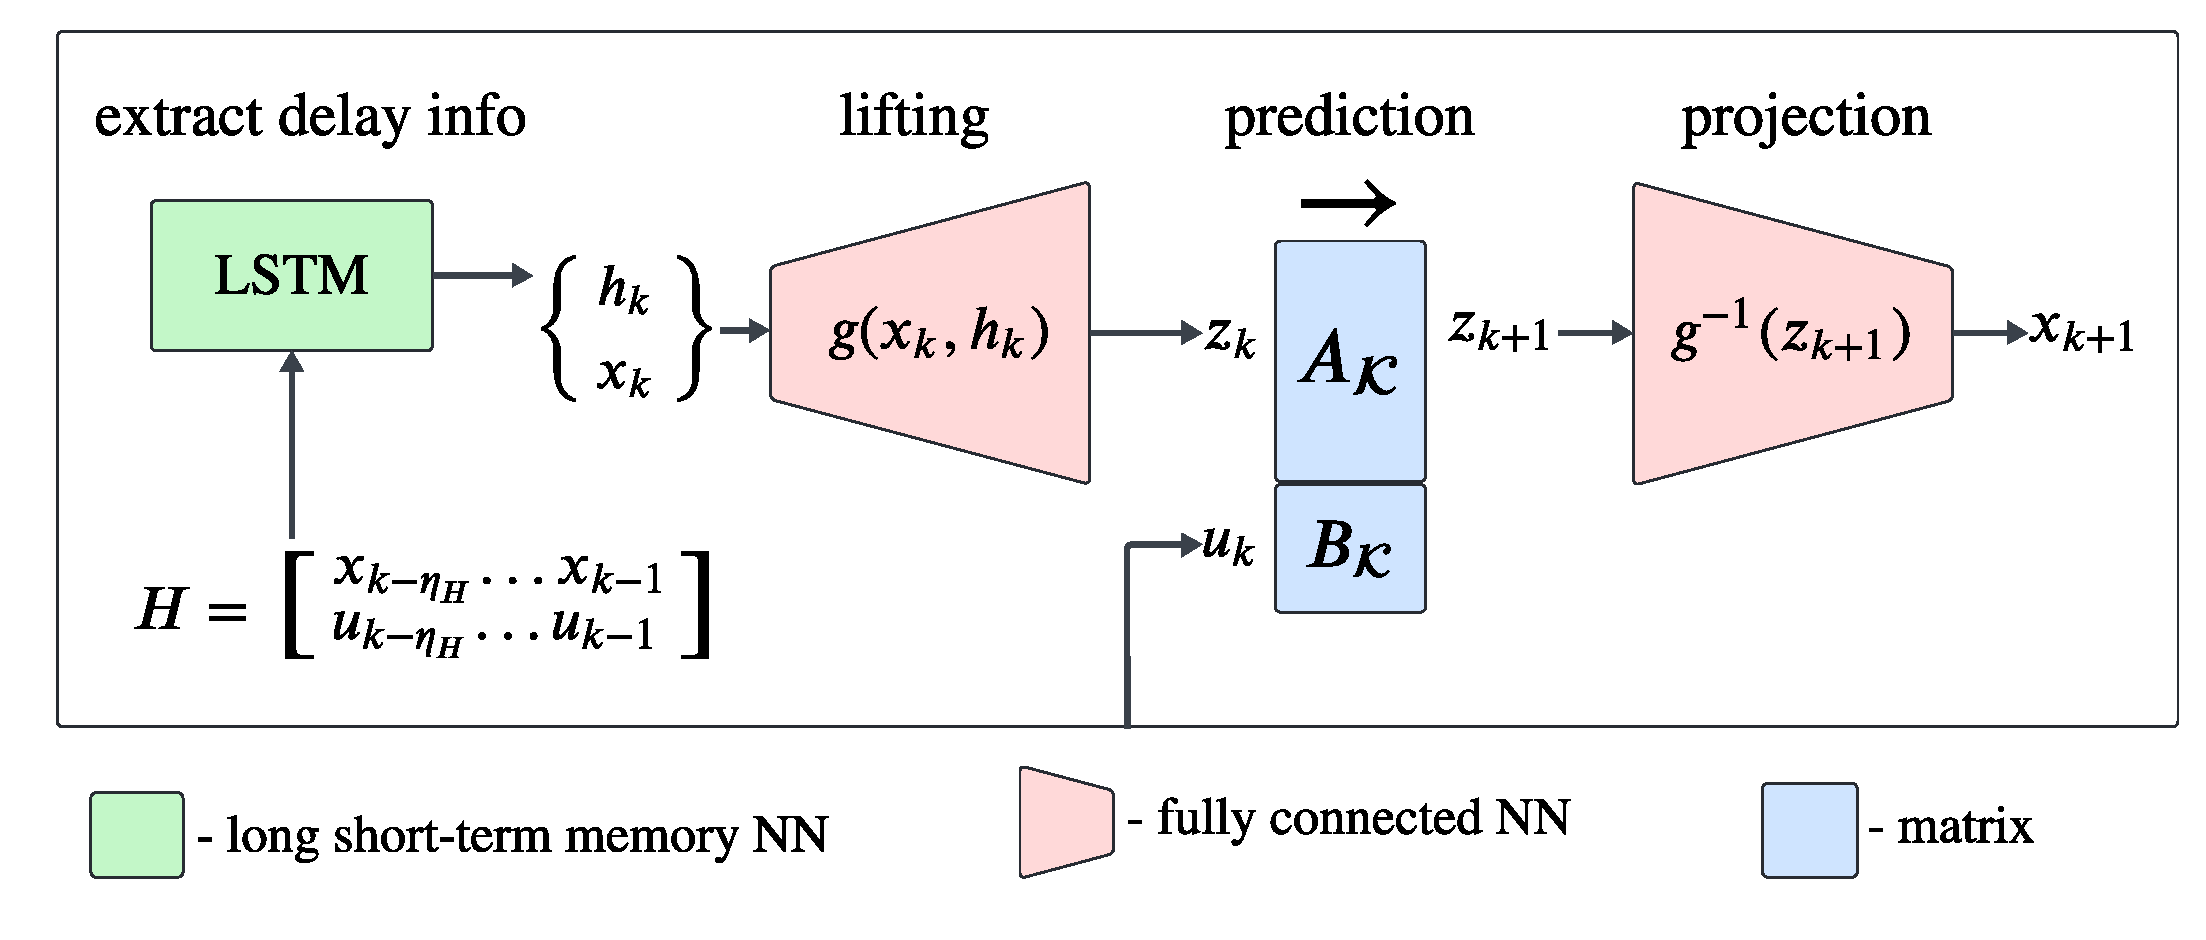
\includegraphics[width = \linewidth]{figures/derek_scheme.pdf}
	\caption{\todo{The DeReK algorithm architecture. The model is built on the autoencoder architecture of the DKO. The history of state and input data is first extracted using the LSTM layer. The hidden states of the last LSTM layer are then concatenated with the last state as input to the autoencoder part. The autoencoder part remains the same as for the DKO.}}
	\label{fig:derek_scheme}
\end{figure*}
An important aspect of modeling dynamical systems is accounting for time-delays, which are common in many physical and industrial processes. Time-delay can significantly affect system behavior and control performance. Introducing time-delayed embeddings of control action in DMD improves identification of system with input delays, while does not explicitly identify the time-delays. Various methods exist to identify and model time-delays, including state-space realization approaches and correlation analysis. The state-space realization approach involves constructing a state-space representation based on input-output data from experiments, extracting time-delay information from the system's impulse response~\cite{Lima2015254}. Correlation analysis, on the other hand, focuses on identifying time-delays in dynamic processes with disturbances, aiming to improve control accuracy and stability~\cite{Li201792}.

This paper presents a dictionary-free method for learning linear representations of nonlinear systems with input delays using deep neural networks. By leveraging the strengths of deep learning in generating and updating nonlinear transformations, our approach aims to overcome the limitations of traditional Koopman operator methods and provide a robust framework for modeling and controlling nonlinear systems with time-delays. The following sections will delve into the theoretical background, methodological innovations, and practical applications of our approach, guiding the reader through the key challenges and solutions in this domain.

\section{Methodology}



Deep Recurrent Koopman (DeReK) is a novel approach for data-based identification of approximation of the Koopman operator. It can accurately identify the linear model for processes with time delays. Its basis comes from the Deep Koopman Operator (DKO)~\cite{lusch2018deep} approach.

The DeReK is built to approximate the Koopman operator for the systems with time delays. Thanks to the LSTM layer that processes the system's history denoted $H$, we can effectively capture the time delays in the system. Time delays are encoded as the hidden states of the last LSTM layer denoted $h_k$. Thanks to this encoding (hidden states of LSTM), we can obtain the relevant information about the system's past. 

For example, using the LSTM layer, we can obtain the chosen number (this is a hyperparameter) of hidden states. These hidden states are then used as input to the encoder part of our approach. This way, we can reduce the amount of input data to the model compared to the Deep Koopman model, which would take the whole history of the system as input. This would be very inefficient and computationally more expensive.

Also, compared to the DMD, where we would use the history of measurements, we can have a smaller Koopman matrix $\mathcal{K}$. Considering, for example, the last $\ui{l}{his}$ measurements of the system states $x \in \mathbb{R}^n$, the $A_\mathcal{K}$ would have the size $\ui{l}{his}n \times \ui{l}{his}n$ and the $B_\mathcal{K}$ would have the size $\ui{l}{his}n \times m$,  where $m$ is the number of inputs to the system $u \in \mathbb{R}^m$. This is often an unnecessary huge matrix and computationally expensive to compute and store if we are dealing with a long history and many states. On the other hand, the LSTM layer can capture the relevant information about the system's past and reduce the amount of input data in the model.

DRKO, by adding an LSTM layer, processes the history of measurements. As a result, they could better approximate the nonlinear system model with time delay compared to DeSKO. This approach is different from the DeReK, where we are not using the probabilistic neural network or probabilistic recurrent neural networks. Also, the work does not use the autoencoder approach to the model's training; it only uses the NNs to get the probabilistic lifted states.

\subsection{Implementation of Deep Recurrent Koopman (DeReK)}
DeReK was implemented in the Python programming language using the NeuroMANCER~\cite{Neuromancer2023} library. NeuroMANCER stands for Neural Modules with Adaptive Nonlinear Constraints and Efficient Regularizations. It is an open-source differentiable programming (DP) library for solving parametric constrained optimization problems, physics-informed system identification, and parametric model-based optimal control. NeuroMANCER is written in PyTorch and allows for systematically integrating machine learning with scientific computing to create end-to-end differentiable models and algorithms embedded with prior knowledge and physics.

There exists "Learning Stable Deep Koopman Operators" and "Learning Stable Control-oriented Deep Koopman Operators" examples based on~\cite{shi2022deep, korda2020optimal,lusch2018deep} which served as a base for our implementation and comparison of the DeReK model. Also, they provided implementation for learning stable Koopman operator based on Generic Stable Layers~\cite{skomski2021constrained, drgovna2022dissipative, zhang2018stabilizing} for constrained learning of NN. Also, implementing the control input in the model needed to be changed. Both models were implemented with the control input not encoded to be further compatible with Koopman MPC~\cite{korda2018linear}. 

The NeuroMANCER does not provide the use of LSTM layers, so we implemented them into the library. This opens the door to further research and development using this library with LSTM layers. 

The schematic of DeReK architecture can be seen in Fig.~\ref{fig:derek_scheme}. The model is built on the autoencoder architecture of the DKO. The history of state and input data is first encoded using the LSTM layer. The hidden states of the last LSTM layer are then concatenated with the last state as input to the autoencoder part. The autoencoder part remains the same as for the DKO.

\subsection{Explicit Loss Function}
In the training of the DeReK model, we are also using the same loss function as in the training of the DKO model. The loss function combines the reconstruction loss, one-step output prediction loss, output trajectory prediction loss, and latent trajectory prediction loss. These loss functions are described in the~\cite{lusch2018deep}. This function is one of the most important parts of the training process. Compared to DMD, where the loss function is only the mean squared error between the predicted and true future states for a one-step prediction, the Deep Koopman methods also use a multi-step prediction in a loss function. In identifying a system, by using the multi-step prediction, we can better capture the system's dynamics with input delays as opposed to only one-step prediction loss.

\paragraph*{Reconstruction loss}
is the mean squared error between the state $x_k$ and the encoded (lifted) and decoded (unlifted) state $g^{-1}(g(x_k))$:
\begin{equation}
    \mathcal{L}_{\text{rec}} = \left\|x_k - g^{-1}(g(x_k))\right\|^2.
\end{equation}
This loss is the basic loss function for the autoencoder part of the model. It ensures that we can correctly encode and decode the state of the system.

\paragraph*{One step output prediction loss}
is the mean squared error between the predicted state $\hat{x}_{k+1}$ and the true state $x_{k+1}$:

\begin{subequations}
    \begin{align}
        \mathcal{L}_{\text{step}} &= \left\|\hat{x}_{k+1} - x_{k+1}\right\|^2, \\
        \hat{x}_{k+1} &= g^{-1}(A_\mathcal{K}g(x_k) + B_\mathcal{K}u_k),
    \end{align}
\end{subequations}
where $u_k$ is the input flow rate at time $k$, the $A_\mathcal{K}$ and $B_\mathcal{K}$ are the identified Koopman matrices.

\paragraph*{Output trajectory prediction loss}
\label{par:output_loss}
is the mean squared error between the predicted trajectory $\hat{x}_{k+1:k+N}$ and the true trajectory $x_{k+1:k+N}$:
\begin{subequations}
    \begin{align}
        \mathcal{L}_{\text{pred}} &= \sum_{i=1}^{N}\left\|\hat{x}_{k+i} - x_{k+i}\right\|^2, \\
        \hat{x}_{k+i} &= g^{-1}\left(A_\mathcal{K}g(\hat{x}_{k+i-1}) + B_\mathcal{K}u_{k+i-1}\right), \\
        \hat{x}_{k} &= x_{k},
    \end{align}
\end{subequations}
where $N$ is the prediction horizon specified by a user. In this case, the predicted trajectory $\hat{x}_{k:k+N}$ is predicted based on the $x_k$ and the input trajectory $u_{k:k+N-1}$. This loss function is used to capture the dynamics of the system and also input delays. By using the multi-step prediction loss, we can better capture the dynamics of the system as opposed to only one-step prediction loss.

\paragraph*{Latent trajectory prediction loss}
is the mean squared error between the lifted predicted trajectory $\hat{z}_{k+1:k+N}$ and the lifted true trajectory $z_{k+1:k+N}$:
\begin{subequations}
    \begin{align}
        \mathcal{L}_{\text{lpred}} &= \sum_{k=1}^{N}\left\|\hat{z}_{k+i} - z_{k+i}\right\|^2, \\
        z_{k+i} &= g(x_{k+i}), \\
        \hat{z}_{k+i} &= A_{\mathcal{K}}\hat{z}_{k+i-1}+B_{\mathcal{K}}u_{k+i-1},\\
        \hat{z}_{k} &= g(x_{k}),
    \end{align}
\end{subequations}
where this loss function works with the same principle as the output trajectory prediction loss~\ref{par:output_loss}, but in the space of lifted states.

The final loss function is a weighted sum of all the loss functions:
\begin{equation}
    \mathcal{L} = \ui{w}{rec}\mathcal{L}_{\text{rec}} + \ui{w}{step}\mathcal{L}_{\text{step}} + \ui{w}{pred}\mathcal{L}_{\text{pred}} + \ui{w}{lpred}\mathcal{L}_{\text{lpred}},
\end{equation}
where $\ui{w}{rec}$, $\ui{w}{step}$, $\ui{w}{pred}$, and $\ui{w}{lpred}$ are the weights for the reconstruction loss, one-step output prediction loss, output trajectory prediction loss, and latent trajectory prediction loss, respectively. They are set by the user and are used to balance the importance of the loss functions in the training process.


\section{Results}

\subsection{Comparison with eDMD}

Here we compare the performance of DeReK with eDMD on a simulated two tank system without interaction with an input delays. The system is described by the following equations:

\begin{equation}\label{eq:two_tanks_system}
    \begin{aligned}
        \diff{h_1(t)}{t} & = q(t-\tau) - \frac{k_1}{F_1}\sqrt{h_1(t)}                     \\
        \diff{h_2(t)}{t} & = \frac{k_1}{F_2}\sqrt{h_1(t)} - \frac{k_2}{F_2}\sqrt{h_2(t)},
    \end{aligned}
\end{equation}

where \(h_1(t)\) and \(h_2(t)\) are the water levels in tanks 1 and 2, respectively, \(q(t)\) is the input flow rate, \(\tau \) is the input delay, and \(k_1\), \(k_2\) are the flow rate constants of the valves and \(F_1\), \(F_2\) are the cross-sectional areas of the tanks.

The experimental data were acquired by simulating this system at sampling period \( \ui{T}{s} = 10 \, \mathrm{s} \) with input delay \( \tau = 2\ui{T}{s} \). Random change in the input flow rate from the interval \( \ui{q}{min} = 0.0 \, \text{m}^3\text{s}^{-1} \), \( \ui{q}{max} = 0.03 \) \( \text{m}^3\text{s}^{-1} \) was applied to the system.

The data were split into training and testing sets with a ratio of 50:50. The training set was used to train the models, while the testing set was used to evaluate their performance. The models were trained to predict the water levels in tanks 1 and 2 for the whole testing set based on the applied input flow rate and the initial state of the system.

eDMD used dictionary of polynomials up to degree 2, square root and inversion of the water levels, and time-delayed embeddings of the input flow rate composed of previous 20 samples. Lifted states were obtained by concatenating the dictionary terms and time-delayed embeddings, and the Koopman matrix was learned using eDMD.

The DeReK model consists of an LSTM layer with one hidden layer with 8 units, to extracts information about the time delays in the system from the history of the system. The concatenated information is then transformed to lifted states using an encoder layer with a fully connected network. The lifted states are further concatenated with the input flow rate using another concatenation layer.

Figure~\ref{fig:two_tanks_results} shows the predicted and actual water levels in tanks 1 and 2 for the two tank system using eDMD and DeReK. The results demonstrate that DeReK outperforms eDMD in terms of prediction accuracy, capturing the system's dynamics more effectively over the testing set. eDMD exhibits systematic positive bias in the prediction of water levels, while DeReK provides more accurate and consistent predictions. Nevertheless, the linear model generated by DeReK displays non-minimum phase behavior, which is a common issue in identification of systems with input delays.

\begin{figure}[htbp]\label{fig:two_tanks_results}
    \centerline{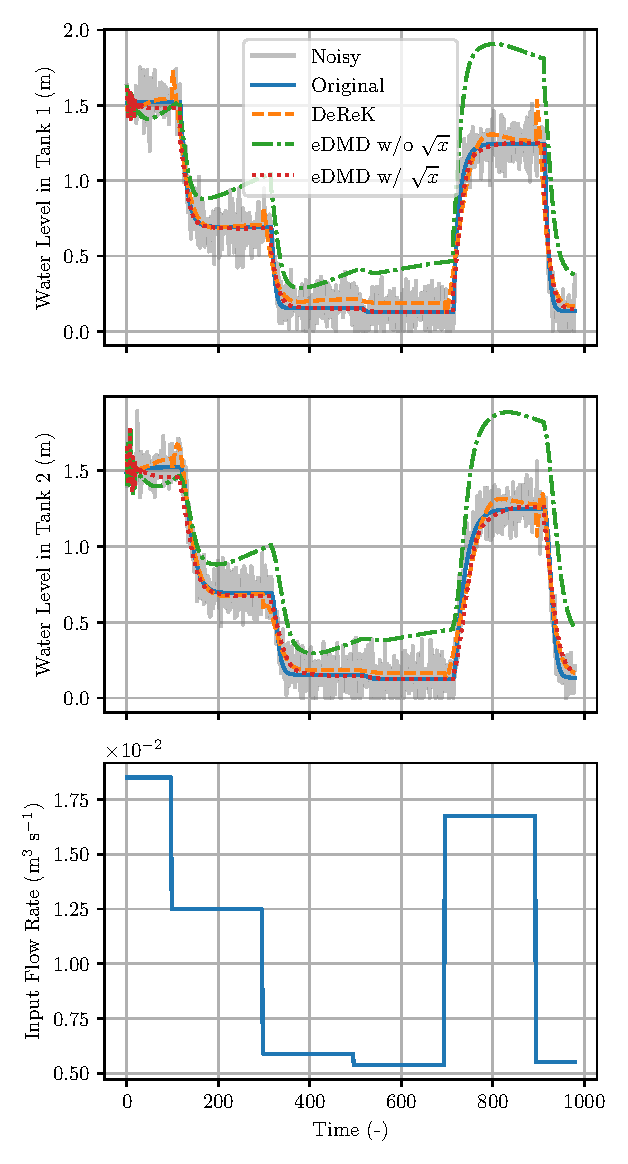
\includegraphics[width=\linewidth]{figures/dmdc_multipred-p0-q0-hm20-hl0.pdf}}
    \caption{Predicted and actual water levels in tanks 1 and 2 for the two tank system}
\end{figure}

The performance of the models was evaluated using the mean absolute error (MAE) and the sum of the absolute differences (SAD) between the predicted and actual water levels in tanks 1 and 2. The results are presented in Table~\ref{tab:two_tanks_results}. DeReK achieved a significantly lower MAE and SAD compared to eDMD, indicating its superior performance in modeling the two tank system with input delays.

\begin{table}[htbp]\label{tab:two_tanks_results}
    \caption{Performance comparison of DeReK and eDMD on the two tank system with input delays}
    \begin{center}
        \begin{tabular}{c| S[table-format=1.4] S[table-format=3.2]}
            \toprule
            \textbf{Model}              & \textbf{MAE} & \textbf{SAD} \\
            \midrule
            eDMD (with \(\sqrt{x}\))    & 0.1737       & 170.24       \\
            eDMD (without \(\sqrt{x}\)) & 0.6058       & 593.70       \\
            DeReK                       & 0.2005       & 196.51       \\
            \bottomrule
        \end{tabular}
    \end{center}
\end{table}



\bibliographystyle{IEEEtran}
\bibliography{main}

\end{document}
